\documentclass[]{article}
% packages
%\usepackage[utf8]{vietnam}
\usepackage{amsmath, amssymb, amsthm}
\usepackage{color, graphicx, cases}
\usepackage{hyperref}
\hypersetup{
	colorlinks=true,
	linkcolor=black,
	filecolor=black,      
	urlcolor=black,
}
\usepackage{array, multirow, booktabs}
\usepackage{caption, subcaption}
\usepackage{ragged2e} % using justifying
\numberwithin{equation}{section}
\everymath{\displaystyle}
\usepackage{titling}

\usepackage[a4paper,left=35mm,top=31mm,right=20mm,bottom=30mm]{geometry}
\renewcommand{\baselinestretch}{1.5}

% new definitions
\newtheorem{dl}{Theorem}[section]
\newtheorem{md}{Proposition}[section]
\newtheorem{hq}{Corollary}[section]
\newtheorem{cy}{Remark}[section]

\theoremstyle{definition}
\newtheorem{dn}{Definition}[section]
\newtheorem{vd}{Example}[section]
\newtheorem{bt}{Problem}[section]
\newtheorem{nx}{Comment}[section]

% reference
\usepackage{cleveref}
\crefname{dl}{\textbf{Theorem}}{}
\crefname{md}{\textbf{Proposition}}{}
\crefname{hq}{\textbf{Corollary}}{}

\crefname{dn}{\textbf{Definition}}{}
\crefname{vd}{\textbf{Example}}{}
\crefname{cy}{\textbf{Remark}}{}
\crefname{bt}{\textbf{Problems}}{}
\crefname{nx}{\textbf{Comment}}{}
\everymath{\displaystyle}

\title{Reconstruction of a term in the right-hand side of parabolic equations}

\author{Ta Thi Thanh Mai\thanks{email: mai.tathithanh@hust.edu.vn} \and Ho Duc Nhan\thanks{email: hdnhan28@gmail.com}}

\thanksmarkseries{arabic}
\date{\footnotesize\textit{School of Applied Mathematics and Informatics, Hanoi University of Science and Technology, \\ No.1 Dai Co Viet street, Hai Ba Trung District, Hanoi, Vietnam}}

\begin{document}
\justifying
\maketitle
%\thispagestyle{empty}
%\normalsize
\begin{abstract}
	...
\end{abstract}
\textbf{Keywords:} Inverse source problems, least squares method, Tikhonov regularization, space-time finite element method, conjugate gradient method.
\section{Introduction}
Consider a physical domain $\Omega \subset \mathbb{R}^d,\, d\in \mathbb{N^+}$ be bounded with the boundary $\Gamma$ and donate the cylinder $Q=\Omega\times (0,\, T]$ and lateral surface area $S=\Gamma \times (0,\, T]$ where $T>0$. 
\\
Consider the heat equation
\begin{align}\label{1.1}
	\frac{\partial u}{\partial t}-\sum_{i, j=1}^{d}\frac{\partial}{\partial x_j}\left(a_{ji}(x, t)\frac{\partial u}{\partial x_i}\right)=F(x, t), \quad(x, t)\in Q,
\end{align}
with the initial and Dirichlet conditions, respectively
\begin{align}
	u(x, 0)&=u_0(x),\quad x\in \Omega,\label{1.2}\\
	u(x, t)&=0,\quad(x, t)\in S, \label{1.3}
\end{align}
where
\begin{align*}
	&a_{ij}\in L^{\infty}(Q),\, a_{ij}=a_{ji},\; \forall i, j\in \{1, 2, ..., d\},\\
	&\lambda_1\left\|\xi\right\|^2\leq \sum_{i, j=1}^{d}a_{ij}\xi_i\xi_j\leq \lambda_2\left\|\xi\right\|^2,\; \forall \xi\in\mathbb{R}^d,\\
	&u_0\in H^1_0(\Omega),\; F\in L^2(0,\, T;\, H^{-1}(\Omega)),
\end{align*}
with $\lambda_1$ và $\lambda_2$ are positive constants.
\\
The direct problem is to determine $u$ when all data $a_{ji}, i, j=\overline{1, d}, \,u_0, \,\varphi$ and $F$ in \cref{1.1,1.2,1.3} are given. On the other hand, the inverse problem (IP) is to identify a missed data such as the right hand side $F$ when some additional observations on the solution $u$ are available. 
\\
We consider the right hand side of the equation \eqref{1.1} following the form $F(x, t)=f(.)q(x, t)+g(x, t)$, where $q(x, t),\, g(x, t)$ are given and $f(.)$ can be either $f(x, t)$, $f(x)$ or $f(t)$.
%Denote $N_m$ is the number of measurements and $\ell_k u(f) =\omega_k, k=\overline{1, N_m}$ is the value of the $kth$ measurement. 
We have different inverse problems depending on either the form of $F$ or the observation on the solution $u$: 
\begin{itemize}
	\item IP1: Find $f(x, t)$ if $u(x, t)$ is given on $Q$ \cite{a1, a2}.
	\item IP2: Find $f(x)$ if $u(x, T)$ is given on $\Omega$ \cite{a3, a4, a5, a6}.
	\item IP3: Find $f(t)$ if $\int_\Omega w(x)u(x, t)dx$ and $w(x)>0, \forall x\in \Omega$ are given \cite{a7, a8, a9}. This observation called \textit{integral observation}. Furthermore, an observation derives from integral observation called \textit{point observation} if $w(x)$ is a dirac delta function $\delta(x-x_0)$, so that $\int_\Omega\delta(x-x_0)u(x, t)dx=u(x_0, t), x_0$ is a point in $\Omega$ \cite{a10, a11, a12}. Beside that, find $f(x, t)$ or $f(x)$ if some integral or point observations are available \cite{a13}.
	%\item IP3: Find $f(t)$ if $\ell_ku=\int_\Omega w_k(x)u(x, t)dx=\omega_k(t)$ and $w_k(x)>0, \forall x\in \Omega$ are given. This observation called \textit{integral observation}. Furthermore, an observation derives from integral observation called \textit{point observation} if $w_k(x)$ is a dirac delta function $\delta_k(x-x_k)$, so that $\ell_k(t)=\int_\Omega\delta_k(x-x_k)u(x, t)dx=u(x_k, t)=\omega_k(t)$. 
\end{itemize}
Donate $w$ is the value of the observation that given and $\ell u(f)$ is the result of the observation based on the solution $u$ we get. In this paper, we only present  the case of having many integral observations with $N_m$ is the number of observations, others can be proved similarly. So, to solve this problem, we need to minimize the least square functional \cite{a14, a15}
$$J_{\gamma}(f)=\frac{1}{2}\sum_{k=1}^{N_{m}}\left\|\ell_k u(f)-\omega_k\right\|_{L^2(0, T)}^2.$$
However, this minimization problem is unstable and there might be many minimizers to it. Therefore, we minimize the Tikhonov functional instead
$$J_{\gamma}(f)=\frac{1}{2}\sum_{k=1}^{N_{o}}\left\|\ell_k u(f)-\omega_k\right\|_{L^2(0, T)}^2+\frac{\gamma}{2}\left\|f-f^*\right\|_{*}^2,$$
with $\gamma>0$ being a regularization parameter, $f^*$ is an a prior estimation of $f$ and $\left\|.\right\|_*$ an appropriate norm.

\section{Variational problem}
To introduce the concept of weak form, we use the standard Sobolev spaces $H^1(\Omega),\, H^1_0(\Omega),\, H^{1, 0}(Q)$ and $H^{1, 1}(Q)$ \cite{b1, b2, b3}. Further, for a Banach space $B$, we define
$$L^2(0, T; B)=\left\{u:u(t)\in B \text{ a.e } t\in (0, T) \text{ and } \left\|u\right\|_{L^2(0, T;\; B)} <\infty \right\},$$
with the norm
$$\left\|u\right\|_{L^2(0, T; B)}^2=\int_0^T\left\|u(t)\right\|^2_Bdt.$$
In this paper, we will use an equivalent norm in $L^2\left(0, T; H^1_0(\Omega)\right)$ with the norm
$$\left\|u\right\|_{L^2(0, T;\; H^1_0(\Omega))}^2=\int_Q \sum_{i, j=1}^{d}a_{ji}\frac{\partial u}{\partial x_i}\frac{\partial u}{\partial x_j}dxdt.$$
So, with the duality pairing $\langle ., .\rangle_Q$, the dual norm will be
$$\left\|u\right\|_{L^2(0, T;\; H^{-1}(\Omega))}=\sup_{0\neq v\in L^2(0, T;\; H^1_0(\Omega))}\frac{\langle u, v\rangle_Q}{\left\|v\right\|_{L^2(0, T;\; H^1_0(\Omega))}}.$$
In the sequel, we shall use the space $W(0, T)$ define as
$$W(0, T)=\left\{u: u\in L^2(0, T; H^1_0(\Omega)), u_t\in L^2\left(0, T; H^{-1}(\Omega) \right)\right\}$$
A week solution in $W(0, T)$ of the problem \cref{1.1,1.2,1.3} is a function $u(x, t)\in W(0, T)$ satisfying the identity
\begin{align}\label{2.1}
	\int_{Q}\left[\frac{\partial u}{\partial t}v+\sum_{i, j=1}^{d}a_{ji}\frac{\partial u}{\partial x_i}\frac{\partial v}{\partial x_j}\right]dxdt=\int_{Q}Fvdxdt,\;\forall v \in L^2\left(0, T; H^1(\Omega)\right).
\end{align}
or 
\begin{align*}
	a(u, v)=\langle F, v\rangle_{Q},\;\forall v \in L^2\left(0, T; H^1_0(\Omega)\right).
\end{align*}
and 
\begin{align}\label{2.2}
	u(x, 0)=u_0,\; x\in \Omega.
\end{align}
From now on, we donate $X=\left\{u: u\in W(0, T): u(x, 0)=0\right\}$ and $Y=L^2\left(0, T; H^1_0(\Omega)\right)$. Obviously, we have $X\subset Y$. We split $u(x, t)=\overline{u}(x, t)+\overline{u}_0$ for $(x, t)\in Q$ where $\overline{u}_0\in W(0, T)$ is some extension of the given initial datum $u_0\in H^1_0(\Omega)$. Here, we use space-time finite element method \cite{a16} and therefore we can prove that there exists a unique solution $\overline{u}\in X$ of the problem \cref{1.1,1.2,1.3} that satisfies 
\begin{align}\label{2.3}
	\left\|\overline{u}\right\|_{W(0, T)} \leq c_d \left(\left\|F\right\|_{L^2\left(0, T; H^{-1}(\Omega)\right)}+\left\|\overline{u}_0\right\|_{W(0, T)}\right).
\end{align}
We suppose that $F$ has the form $F(x, t)=f(x, t)q(x, t)+g(x, t)$ with \color{red} $f\in L^2(Q),\, q\in L^\infty(Q)$ and $g\in L^2(Q)$\color{black}. We hope to recover $f(x, t)$ from the observation. Since the solution $u(x, t)$ depends on the function $f(x, t)$, so we denote it by $u(x, t, f)$ or $u(f)$. Identify $f(x, t)$ satisfying 
$$\ell_k u(f)=\omega_k,\; \forall k = \overline{1, N_m}.$$
%where $\ell_k u(f)$ is the observation on the solution depending on $f$. We suppose to solve (IP2) problem and (IP1) will be done the same way. 
We need to minimize the Tikhonov functional
\begin{align}\label{2.4}
	J_{\gamma}(f)=\frac{1}{2}\sum_{k=1}^{N_m}\left\|\ell_k u(f)-\omega_k\right\|_{L^2(0, T)}^2+\frac{\gamma}{2}\left\|f-f^*\right\|_{L^2(Q)}^2.
\end{align}
We will prove that $J_\gamma$ is Frechet differentiable and drive a formula for its gradient. In doing so, we need the adjoint problem
\begin{align}\label{2.5} 
	\begin{cases}
		-\frac{\partial p}{\partial t}-\sum_{i, j=1}^{d}\frac{\partial}{\partial x_j}\left(a_{ji}(x, t)\frac{\partial p}{\partial x_i}\right)=\sum_{k=1}^{N_m}w(x)\left(\ell_k u(f)-\omega_k\right), & (x, t)\in Q,\\
		u(x, t)=0, & (x, t)\in S\\
		p(x, T)=0, & x\in \Omega.
	\end{cases}
\end{align}
By changing the time direction, meaning $\tilde{p}(x, t)=p(x, T-t)$, we will get a Dirichlet problem for parabolic equations.
\begin{dl}
	The functional $J_\gamma$ is Frechet differentiable and its gradient $\nabla J_\gamma$ at $f$ has the form 
	\begin{align}\label{2.6}
		\nabla J_\gamma(f)=q(x, t)p(x, t)+\gamma \left(f(x, t)-f^*(x, t)\right)
	\end{align}
\end{dl}
\begin{proof}
	By taking a small variation $\delta f \in L^2(Q)$ of $f$ and denoting $\delta u(f)=u(f+\delta f)-u(f)$, we have
	\begin{align*}
		J_0(f+\delta f)-J_0(f)&=\frac{1}{2}\sum_{k=1}^{N_m}\left\|\ell_k u(f+\delta f)-\omega_k\right\|^2_{L^2(0, T)}-\frac{1}{2}\sum_{k=1}^{N_m}\left\|\ell_k u(f)-\omega_k\right\|^2_{L^2(0, T)}\\
		&=\frac{1}{2}\sum_{k=1}^{N_m}\left\|\ell_k \delta u(f) +\ell_k u(f)-\omega_k\right\|^2_{L^2(0, T)}-\frac{1}{2}\sum_{k=1}^{N_m}\left\|\ell_k u(f)-\omega_k\right\|^2_{L^2(0, T)}\\
		&=\sum_{k=1}^{N_m}\frac{1}{2}\left\|\ell_k \delta u(f)\right\|^2_{L^2(0, T)}+\sum_{k=1}^{N_m}\left\langle \ell_k \delta u(f), \ell_k u(f)-\omega_k\right\rangle_{L^2(0, T)},
	\end{align*}
	where $\delta u(f)$ is the solution to this problem
	\begin{align}\label{2.7}
		\begin{cases}
			\frac{\partial \delta u}{\partial t}-\sum\limits_{i, j=1}^{d}\frac{\partial}{\partial x_j}\left(a_{ji}(x, t)\frac{\partial \delta u}{\partial x_i}\right)=q(x, t)\delta f,&(x, t)\in Q,\\
			\delta u(x, t)=0, & (x, t)\in S,\\
			\delta u(x, 0)=0, &x\in \Omega.
		\end{cases}
	\end{align}
	Because the priori estimate \eqref{2.3} for the direct problem, we have
	\begin{align}\label{2.8}
		\left\|\ell_k\delta u(f)\right\|_{L^2(0, T)}^2=o\left(\left\|\delta f\right\|_{L^2(Q)}\right)\, \text{when } \left\|\delta f\right\|_{L^2(Q)}\to 0.
	\end{align}
	What is more, applying the Green formula [...] for \eqref{2.5} and \eqref{2.7}, we get
	\begin{align}\label{2.9}
		\sum_{k=1}^{N_m}\int_{Q} \delta u(x, t) w(x) \left(\ell_k u(f)-\omega_k(t)\right)dxdt=\int_{Q} p(x, t)q(x, t)\delta f(x, t)dxdt
	\end{align}
	According to \eqref{2.8} and \eqref{2.9}, we obtain
	\begin{align*}
		J_0(f+\delta f)-J_0(f)&=\sum_{k=1}^{N_m}\int_{Q}\delta u(x, t)w(x)\left(\ell_k u(f)-\omega_k(t)\right)ds+o\left(\left\|\delta f\right\|_{L^2(Q)}\right)\notag\\
		&=\int_Q q(x, t)p(x, t)\delta f(x, t)dxdt+o\left(\left\|\delta f\right\|_{L^2(I)}\right)\notag\\
		&=\left\langle qp,\delta f \right\rangle_{L^2(Q)}+o\left(\left\|\delta f\right\|^2_{L(Q)}\right).
	\end{align*}
	Therefore, we will obtain
	$$J_\gamma(f+\delta f)-J_\gamma(f)=\left\langle qp,\delta f \right\rangle_{L^2(Q)}+\gamma\left\langle f-f^*,\delta f \right\rangle_{L^2(Q)}+o\left(\left\|\delta f\right\|^2_{L(Q)}\right).$$
	Hence the functional $J_\gamma$ is Frechet differentiable and its gradient $\nabla J_\gamma$ at $f$ has the form \eqref{2.6}. The theorem is proved.
\end{proof}
\begin{cy}
	In this theorem, we write the Tikhonov functional for $F(x, t)=f(x, t)q(x, t)+g(x, t)$. But when F has another form, the penalty term should be modified
	\begin{itemize}
		\item $F(x, t)=f(x)q(x, t)+g(x, t)$: the penalty functional is $\left\|f-f^*\right\|_{L^2(\Omega)}$ and $$\nabla J_0(f)=\int_0^Tq(x, t)p(x, t)dt.$$
		\item $F(x, t)=f(t)q(x, t)+g(x, t)$: the penalty functional is $\left\|f-f^*\right\|_{L^2(0, T)}$ and $$\nabla J_0(f)=\int_\Omega q(x, t)p(x, t)dt.$$
	\end{itemize}
\end{cy}
\noindent To find $f$ satisfied \eqref{2.4}, we use the conjugate gradient method (CG). Its iteration follows, we assume that at the $k$th iteration, we have $f^k$ and then the next iteration will be
$$f^{k+1}=f^k+\alpha_kd^k,$$
with
\begin{align*}
	d^k&=\left\{\begin{array}{ll}
	-\nabla J_\gamma(f^k),& k=0,\\
	-\nabla J_\gamma(f^k)+\beta_kd^{k-1},& k>0,
	\end{array}\right.\\\\
	\beta_k&=\frac{\left\|\nabla J_\gamma (f^k)\right\|^2_{L^2(I)}}{\left\|\nabla J_\gamma (f^{k-1})\right\|^2_{L^2(I)}},
\end{align*}
and
$$\alpha_k=\operatorname*{arg\,min}_{\alpha\geq 0}J_\gamma(f^k+\alpha d^k).$$
To identify $\alpha_k$, we consider two problems
\begin{bt}\label{bt2.1}
	Denote the solution of this problem is $u[f]$
	\begin{align*}
		\begin{cases}
			\frac{\partial u}{\partial t}-\sum_{i, j=1}^{d}\frac{\partial}{\partial x_j}\left(a_{ji}(x, t)\frac{\partial u}{\partial x_i}\right)=f(x, t)q(x, t),&(x, t)\in Q,\\
			u(x, t)=0, & (x, t)\in S,\\
			u(x, 0)=0,&x\in \Omega.
		\end{cases}
	\end{align*}
\end{bt}
\begin{bt}\label{bt2.2}
	Denote the solution of this problem is $u(u_0, \varphi)$
	\begin{align*}
		\begin{cases}
			\frac{\partial u}{\partial t}-\sum_{i, j=1}^{d}\frac{\partial}{\partial x_j}\left(a_{ji}(x, t)\frac{\partial u}{\partial x_i}\right)=g(x, t),&(x, t)\in Q,\\
			u(x, t)=0, & (x, t)\in S,\\
			u(x, 0)=u_0(x),&x\in \Omega.
		\end{cases}
	\end{align*}
\end{bt}
\noindent If we do so, the observation operators have the form $\ell_i u(f)=\ell_i u[f]+\ell_i u(u_0, \varphi)=A_if+\ell_i u(u_0, \varphi)$, with $A_i$ being bounded linear operators from $L^2(Q)$ to $L^2(0, T)$.\\
We have
\begin{align*}
	J_{\gamma}(f^k+\alpha d^k)&=\frac{1}{2}\sum_{i=1}^{N_m}\left\|\ell_i u(f^k+\alpha d^k)-\omega_i\right\|_{L^2(0, T)}^2+\frac{\gamma}{2}\left\|f^k+\alpha d^k-f^*\right\|_{L^2(Q)}^2\\[0.2cm]
	&=\frac{1}{2}\sum_{i=1}^{N_m}\left\|\alpha A_id^k+A_if^k+\ell_i u(u_0, \varphi)-\omega_i\right\|_{L^2(0, T)}^2+\frac{\gamma}{2}\left\|f^k+\alpha d^k-f^*\right\|_{L^2(Q)}^2\\[0.2cm]
	&=\frac{1}{2}\sum_{i=1}^{N_m}\left\|\alpha A_id^k+\ell_i u(f^k)-\omega_i\right\|_{L^2(0, T)}^2+\frac{\gamma}{2}\left\|f^k+\alpha d^k-f^*\right\|_{L^2(Q)}^2.
\end{align*}
Differentiating $J_\gamma(f^k+\alpha d^k)$ with respect to $\alpha$, we get
\begin{align*}
	\frac{\partial J_\gamma(f^k+\alpha d^k)}{\partial \alpha} &= \alpha\sum_{i=1}^{N_m}\left\|A_id^k \right\|_{L^2(0, T)}^2+\sum_{i=1}^{N_m}\left\langle A_id^k,\ell_i u(f^k)-\omega_i\right\rangle_{L^2(0, T)}\\[0.2cm]
	&\quad+\gamma\alpha\left\| d^k\right\|_{L^2(Q)}^2+\gamma\left\langle d^k, f^k-f^*\right\rangle_{L^2(Q)}.
\end{align*}
Putting $\frac{\partial J_\gamma(f^k+\alpha d^k)}{\partial \alpha}=0$, we obtain
\begin{align*}
	\alpha_k&=-\frac{\displaystyle\sum_{i=1}^{N_m}\left\langle A_id^k, \ell_i u(f^k)-\omega_i\right\rangle_{L^2(0, T)}+\gamma\left\langle d^k, f^k-f^*\right\rangle_{L^2(Q)}}{\displaystyle\sum_{i=1}^{N_m}\left\|A_id^k\right\|^2_{L^2(0, T)}+\gamma\left\|d^k\right\|^2_{L^2(Q)}}\\[0.2cm]
	&=-\frac{\displaystyle\sum_{i=1}^{N_m}\left\langle d^k, A_i^*\left(\ell_i u(f^k)-\omega_i\right)\right\rangle_{L^2(Q)}+\gamma\left\langle d^k, f^k-f^*\right\rangle_{L^2(Q)}}{\displaystyle\sum_{i=1}^{N_m}\left\|A_id^k\right\|^2_{L^2(0, T)}+\gamma\left\|d^k\right\|^2_{L^2(Q)}}\\[0.2cm]
	&=-\frac{\displaystyle\sum_{i=1}^{N_m}\left\langle d^k, A_i^*\left(\ell_i u(f^k)-\omega_i\right)+\gamma(f^k-f^*)\right\rangle_{L^2(Q)}}{\displaystyle\sum_{i=1}^{N_m}\left\|A_id^k\right\|^2_{L^2(0, T)}+\gamma\left\|d^k\right\|^2_{L^2(Q)}}\\[0.2cm]
	&=-\frac{\left\langle d^k,\nabla J_\gamma(f^k)\right\rangle_{L^2(Q)}}{\displaystyle\sum_{i=1}^{N_m}\left\|A_id^k\right\|^2_{L^2(0, T)}+\gamma\left\|d^k\right\|^2_{L^2(Q)}}.
\end{align*}
Because of $d^k=r^k+\beta_kd^{k-1},\, r^k=-\nabla J_\gamma (f^k)$ and $\left\langle r^k,d^{k-1}\right\rangle_{L^2(I)}=0$, we get 
$$\alpha_k=\frac{\left\|r^k\right\|^2_{L^2(Q)}}{\displaystyle\sum_{i=1}^{N_m}\left\|A_id^k\right\|^2_{L^2(0, T)}+\gamma\left\|d^k\right\|^2_{L^2(Q)}}.$$

\noindent \textbf{CG algorithm}
\begin{itemize}
	\item[1.] Set $k=0$, initiate $f^0$.
	\item[2.] For $k=0, 1, 2,...$. Calculate
	$$r^k=-\nabla J_\gamma(f^k).$$
	Update\\
	\begin{align*}
		d^k&=\left\{\begin{array}{ll}
		r^k,& k=0,\\
		r^k+\beta_kd^{k-1},& k>0,
		\end{array}\right.\\\\
		\beta_k&=\frac{\left\|r^k\right\|^2_{L^2(Q)}}{\left\|r^{k-1}\right\|^2_{L^2(Q)}}.
	\end{align*}
	\item[3.] Calculate
	$$\alpha_k=\frac{\left\|r^k\right\|^2_{L^2(Q)}}{\displaystyle\sum_{i=1}^{N_m}\left\|A_id^k\right\|^2_{L^2(0, T)}+\gamma\left\|d^k\right\|^2_{L^2(Q)}}.$$
	Update
	$$f^{k+1}=f^{k}+\alpha_kd^k.$$
\end{itemize}

\section{Finite element method}
We rewrite the Tikhonov functional
\begin{align*}
	J_\gamma(f)&=\frac{1}{2}\sum_{i=1}^{N_m}\left\|\ell_i u[f]+\ell_i u(u_0, \varphi)-\omega_i\right\|^2_{L^2(0, T)}+\frac{\gamma}{2}\left\|f-f^*\right\|^2_{L^2(Q)}\\
	&=\frac{1}{2}\sum_{i=1}^{N_m}\left\|A_if+\ell_i u(u_0, \varphi)-\omega_i\right\|^2_{L^2(0, T)}+\frac{\gamma}{2}\left\|f-f^*\right\|^2_{L^2(Q)}\\
	&=\frac{1}{2}\sum_{i=1}^{N_m}\left\|A_if-\hat{\omega}_i\right\|^2_{L^2(0, T)}+\frac{\gamma}{2}\left\|f-f^*\right\|^2_{L^2(Q)},
\end{align*}
with $\hat{\omega}_i=\omega_i-\ell_i u(u_0, \varphi)$.
\\
The solution $f^\gamma$ of the minimization problem \eqref{2.4} is characterized by the first-order optimality condition
\begin{align}\label{3.1}
	\nabla J_\gamma(f^\gamma)= \sum_{i=1}^{N_m}A^*_i(A_if^\gamma-\hat{\omega}_i)+\gamma(f^\gamma-f^*)=0,
\end{align}
with $A_i^*: L^2(0, T)\to L^2(Q)$ is the adjoint operator of $A_i$ defined by $\sum_{i=1}^{N_m}A_i^*\left(\ell_i u(f) - \omega_i\right) = p$ where $p$ is the solution of the adjoint problem \eqref{2.5}. 
\\
We will approximate \eqref{3.1} by space-time finite element method. In fact, we will approximate $A_k$ and $A^*_k$ as follows.

\subsection{Finite element approximate of $A_k,\, A_k^*$}
We suppose that finite spaces $W_h\subset W(0, T)$, $X_h \subset X$ and $Y_h \subset Y$, we assume that $X_h \subset Y_h$. 
The Galerkin-Petrov discretization of the variational problem \eqref{2.1} is to find $\overline{u}_h\in X_h$ such that
\begin{align}\label{3.2}
	a(\overline{u}_h, v_h)=\langle F, v_h\rangle_Q-a(\overline{u}_0, v_h), \forall v_h\in Y_h.
\end{align}
For the space-time domain $Q=\Omega\times I\subset \mathbb{R}^{d+1}$, we consider a sequence of admissible decompositions $Q_h$ into shape regular simplicity finite element $q_l$
$$Q_h=\cup_{l=1}^{N}\bar{q}_l.$$
Denote $\left\lbrace (x_k, t_k)\right\rbrace_{k=1}^M $ is a set of nodes $(x_k, t_k)\in \mathbb{R}^{d+1}$. We introduce a reference element $q\in \mathbb{R}^{d+1}$ which any element $q_l$ can maple to $q$ by using
$$\begin{pmatrix}x\\t\end{pmatrix}=\begin{pmatrix}x_k\\t_k\end{pmatrix}+J_l\begin{pmatrix}\xi\\\tau\end{pmatrix}, \; \begin{pmatrix}\xi\\\tau\end{pmatrix}\in q.$$
with $\Delta_l$ is the volume of $q_l$ 
$$\Delta_l=\int_{q_l}dxdt=\det J_l\int_q d\xi d\tau=|q|\det J_l,$$
and the local mesh width
$$h_l=\Delta_l^{\frac{1}{d+1}},\; h:=\max_{l=1, ..., N}h_l.$$
Note that
$$|q|=\begin{cases}
	\frac{1}{2},& d=1,\\[0.1cm]
	\frac{1}{6},& d=2.
\end{cases}$$
The discrete variational problem \eqref{3.2} admits a unique solution $\overline{u}_h\in X_h$. Let $u_h=\overline{u}_h+\overline{u}_{0,h}\in W_h$. Hence, the discrete version of the optimal control problem \eqref{2.4} will be
$$J_{\gamma, h}(f)=\frac{1}{2}\sum_{i=1}^{N_m}\left\|A_{i, h}f-\hat{\omega}_{i, h}\right\|^2_{L^2(0, T)}+\frac{\gamma}{2}\left\|f-f^*\right\|^2_{L^2(Q)}\to \min.$$
Let $f^\gamma_h$ be the solution of this problem is characterized by the variational equation
\begin{align}\label{3.3}
	\nabla J_{\gamma, h}(f^\gamma_h)= \sum_{i=1}^{N_m}A_{i, h}^*(A_{i, h}f^\gamma-\hat{\omega}_{i, h})+\gamma(f^\gamma_h-f^*)=0,
\end{align}
where $A_{i, h}^*$ is the adjoint operator of $A_{i, h}$. But it is hardly to find $A^*_{i, h}$ from $A_{i, h}$ in practice. So we define a proximate $\hat{A}_{i, h}^*$ of $A_i^*$ instead. In deed, we have $\sum_{i=1}^{N_m}\hat{A}^*_{i, h}\phi_i=p_h$, where $\phi_i=\ell_i u(f) - \omega_i$ and $p_h$ is the approximate solution of adjoint problem \eqref{2.5}. Therefore, the equation above will be
\begin{align}\label{3.4}
	\nabla J_{\gamma, h}(f^\gamma_h)\simeq\nabla J_{\gamma, h}(\hat{f}^\gamma_h)= \sum_{i=1}^{N_m}\hat{A}_{i, h}^*(A_{i, h}\hat{f}^\gamma-\hat{\omega}_{i, h})+\gamma(\hat{f}^\gamma_h-f^*)=0,
\end{align}
Moreover, the observation will have noise in practice, so instead of $\omega$, we only get $\omega^{\delta}$ satisfying
$$\left\| \omega-\omega^\delta\right\|_{L^2(S_1)}\leq \delta.$$
Therefore, instead of getting $\hat{f}^\gamma_h$ that satisfies the equation \eqref{3.5}, we will get $\hat{f}^{\gamma, \delta}_h$ satisfying
\begin{align}\label{3.5}
	\nabla J_{\gamma, h}\left(\hat{f}^{\gamma, \delta}_h\right)= \sum_{i=1}^{N_m}\hat{A}_{i, h}^*(A_{i, h}\hat{f}^{\gamma, \delta}_h-\hat{\omega}_{i, h}^\delta)+\gamma(\hat{f}^{\gamma, \delta}_h-f^*)=0,
\end{align}
with $\hat{\omega}_{i, h}^\delta=\omega^\delta-\ell_i u_h(u_0, \varphi)$.
\subsection{Convergence results}
\begin{dl}\label{dl3.2}
	Let $u(x, t)$ be the solution of variational problem \eqref{2.1} - \eqref{2.2} and $\overline{u}_h(x, t)$ be the solution for \eqref{3.2} and $u_h(x, t)=\overline{u}_h(x, t)+\overline{u}_{0, h}(x, t)$. Then there holds the error estimate
	\begin{align}\label{3.6}
		\left\| u-u_h\right\|_{L^2(0, T;\; H^1_0(\Omega))}\leq ch \left|\overline{u}\right|_{H^2(\Omega)}.
	\end{align}
	and 
	\begin{align}\label{3.7}
		\left\| u-u_h\right\|_{L^2(Q)}\leq ch^2 \left|u\right|_{H^2(\Omega)}.
	\end{align}
\end{dl}
\noindent What is more,
\begin{align*}
	\left\| \sum_{i=1}^{N_m}\left(A_i^*-\hat{A}^*_{i,h}\right)\phi_i\right\|_{L^2(Q)}^2=\int_Q (p-p_h)^2dxdt=\left\| p-p_h\right\|_{L^2(Q)}^2
\end{align*}
\begin{align}\label{3.8}
	\Rightarrow \left\| \sum_{i=1}^{N_m}\left(A_i^*-A^*_{i, h}\right)\phi_i\right\|_{L^2(Q)}\leq ch^2.
\end{align}
Let $u_h[f]$ và $u_h(u_0, \varphi)$ are the approximate solutions of \cref{bt2.1} and \cref{bt2.2} by using space-time finite element method. We define $A_h$ of $A$ is $A_hf=\ell u_h[f]$ and $\hat{\omega}_h=\omega-\ell u_h(u_0, \varphi)$. We have
\begin{align*}
	\left\| \sum_{i=1}^{N_m}\left(A_i-A_{i, h}\right)f\right\|_{L^2(0, T)}^2=\sum_{i=1}^{N_m}\left\| \ell_i u[f]-\ell_i u_h[f]\right\|_{L^2(0, T)}^2\leq\sum_{i=1}^{N_m} \left\|w_i\right\|^2_{L^2(\Omega)}\left\| u[f]-u_h[f]\right\|_{L^2(Q)}^2
\end{align*}
\begin{align}\label{3.9}
	\Rightarrow\left\| \sum_{i=1}^{N_m}\left(A_i-A_{i, h}\right)f\right\|_{L^2(0, T)}\leq ch^2
\end{align}
and 
\begin{align*}
	\left\|\sum_{i=1}^{N_m}\left(\hat{\omega}_i-\hat{\omega}_{i, h}\right)\right\|_{L^2(0, T)}^2=\sum_{i=1}^{N_m}\left\| \ell_iu(u_0,\varphi)-\ell_iu_h(u_0, \varphi)\right\|_{L^2(0, T)}^2\leq\sum_{i=1}^{N_m} \left\|w_i\right\|^2_{L^2(\Omega)}\left\| u(u_0,\varphi)-u_h(u_0, \varphi)\right\|_{L^2(Q)}^2
\end{align*}
\begin{align}\label{3.10}
	\Rightarrow\left\|\sum_{i=1}^{N_m}\left(\hat{\omega}_i-\hat{\omega}_{i, h}\right)\right\|_{L^2(0, T)}\leq ch^2
\end{align}

\begin{dl}\label{dl3.3}
	Let $f^\gamma$ and $\hat{f}^\gamma_h$ are the solution of variational problems \eqref{3.1} and \eqref{3.4}, respectively. Then there hold a error estimate
	\begin{align}\label{3.11}
	\left\|f^\gamma-\hat{f}^\gamma_h \right\|_{L^2(Q)}\leq ch^2.
	\end{align}
\end{dl}
\begin{proof} From equations \eqref{3.1} and \eqref{3.4}, we will have
	\begin{align*}
		\gamma \left(f^\gamma-\hat{f}^\gamma_h\right)&=\sum_{i=1}^{N_m}\hat{A}^*_{i, h}\left(A_{i, h}\hat{f}^\gamma_h-\hat{\omega}_{i, h}\right)-\sum_{i=1}^{N_m}A^*_i\left(A_if^\gamma-\hat{\omega}_i\right)\\
		&=\sum_{i=1}^{N_m}\left(\hat{A}^*_{i, h}-A^*_i\right)\left(A_{i, h}\hat{f}^\gamma_h-\hat{\omega}_{i, h}\right)+\sum_{i=1}^{N_m}A^*_iA_{i, h}\left(\hat{f}^\gamma_h-f^\gamma\right)\\
		&\quad+\sum_{i=1}^{N_m}A_i^*\left(A_{i, h}-A_i\right)f^\gamma+\sum_{i=1}^{N_m}A^*_i\left(\hat{\omega}_i-\hat{\omega}_{i, h}\right)
	\end{align*}
	According to \eqref{3.8}, \eqref{3.9} and \eqref{3.10}, we have
	\begin{align*}
		&\left\|\sum_{i=1}^{N_m} \left(\hat{A}^*_{i, h}-A^*_i\right)\left(A_{i, h}\hat{f}^\gamma_h-\hat{\omega}_{i, h}\right)\right\|_{L^2(0, T)}\leq ch^2,\\
		&\left\|\sum_{i=1}^{N_m} A^*_i\left(A_{i, h}-A_i\right)f^\gamma\right\|_{L^2(0, T)}\leq ch^2,\\
		&\left\|\sum_{i=1}^{N_m}A^*_i\left(\hat{\omega}_i-\hat{\omega}_{i, h}\right) \right\|_{L^2(I)}\leq ch^2.
	\end{align*}
	We take apart this
	$$\sum_{i=1}^{N_m}A^*_iA_{i, h}\left(\hat{f}^\gamma_h-f^\gamma\right)=\sum_{i=1}^{N_m}A^*_i\left(A_{i, h}-A_i\right)\left(\hat{f}^\gamma_h-f^\gamma\right)+\sum_{i=1}^{N_m}A^*_iA_i\left(\hat{f}^\gamma_h-f^\gamma\right).$$
	Moreover, we have
	\begin{align*}
		&\left\langle \sum_{i=1}^{N_m}A^*_i\left(A_{i, h}-A_i\right)\left(\hat{f}^\gamma_h-f^\gamma\right), f^\gamma-\hat{f}^\gamma_h\right\rangle_{L^2(0, T)}\leq ch^2\left\| f^\gamma-\hat{f}^\gamma_h\right\|^2_{L^2(Q)},\\
		&\left\langle \sum_{i=1}^{N_m}A^*_iA_i\left(\hat{f}^\gamma_h-f^\gamma\right), f^\gamma-\hat{f}^\gamma_h\right\rangle_{L^2(I)}=-\sum_{i=1}^{N_m}\left\|A_i\left(f^\gamma-\hat{f}^\gamma_h\right) \right\|^2_{L^2(0, T)}<0.
	\end{align*}
	The theorem is proved.
\end{proof}
\begin{cy}\label{cy3.1}
	Let $f^\gamma$ and $\hat{f}^\gamma_h$ are the solution of variational problems \eqref{3.1} and \eqref{3.5}, respectively. Then there hold a error estimate
	\begin{align}\label{3.12}
		\left\|f^\gamma-\hat{f}^{\gamma, \delta}_h \right\|_{L^2(Q)}\leq c(h^2+\delta).
	\end{align}
\end{cy}


\section{Numerical results}
In all examples in this section, we choose the domain $\Omega=(0, 1)\times(0, 1),\, T=1$ and $a_{ij}(x, t)=\delta_{ij}$.
For the temperature we take the exact solution be given by
$$u(x, t)=e^t(x_1-x_1^2)\sin(\pi x_2).$$
We would like to reconstruct function $f$ with several forms of $F$ following
\begin{itemize}
	\item Example 1: $F(x, t)=f(x, t)q(x, t)+g(x, t)$ for IP1 (Example 1.1) with $f(x, t)=\sin(\pi x_1)(x_2-x_2^2)(t^2+1)$,
	\item Example 2: $F(x, t)=f(x)q(x, t)+g(x, t)$ for IP2 (Example 2.1) and IP3 (Example 2.2) with $f(x)=\sin(\pi x_1)(x_2-x_2^2)$,
	\item Example 3: $F(x, t)=f(t)q(x, t)+g(x, t)$ for IP3 with following functions
	\begin{itemize}
		\item[1.]$f(t)=
			\begin{cases}
			2t, & t\in [0, 0.5],\\
			2(1-t), & t \in [0.5, 1],
			\end{cases}$ \qquad for Example 3.1
 		\item[2.] $f(t)=
		\begin{cases}
		1, & t\in [0.25, 0.75],\\
		0, & t \notin [0.25, 0.75],
		\end{cases}$ \qquad for Example 3.2
	\end{itemize}
\end{itemize}
We use a uniform decomposition of the domain $Q$ into $65^3=274,625$ nodes and $6\times 64^3=1,572,864$ finite elements. We take $q(x, t)=x_1x_2+t+1$, initial guess $f^*=0, \gamma=10^{-5}$ and level noise $\delta =1\%$.

\newpage
\noindent\textbf{Example 1.1}
\\
We reconstruct $f(x, t)$ with observation in the whole domain.
\begin{figure}[h!]
	\centering
	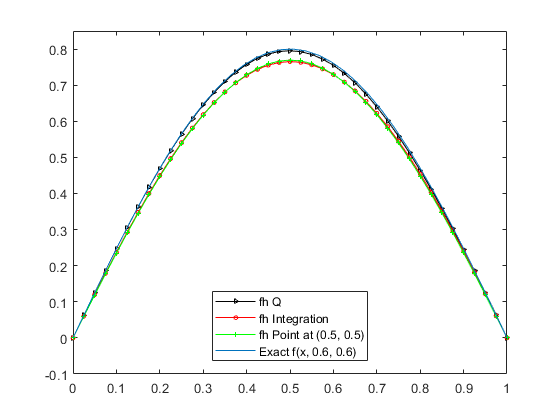
\includegraphics[width=.5\linewidth]{../FreeFem++/fhx}
	\caption{The exact $f(x_p, t),\; x_p=(0.5, 0.5)$ and the numerical solution of Example 1.1.}
\end{figure}

\noindent\textbf{Example 2.1}
\\
We reconstruct $f(x)$ with observation is the final overdetermination.
\begin{figure}[h!]
	\begin{subfigure}{.5\linewidth}
		\centering
		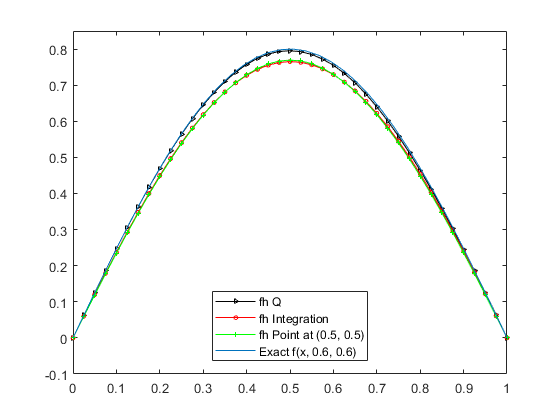
\includegraphics[width=\linewidth]{../FreeFem++/fhx}
	\end{subfigure}%
	\begin{subfigure}{.5\linewidth}
		\centering
		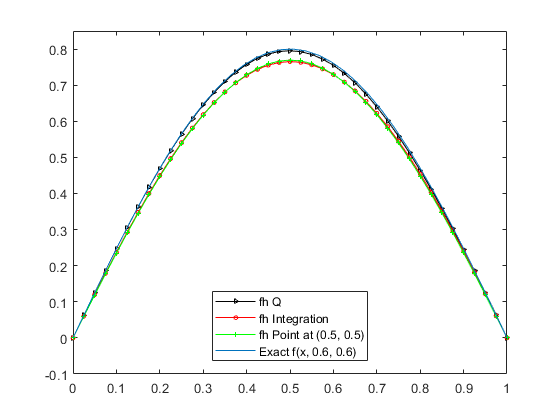
\includegraphics[width=\linewidth]{../FreeFem++/fhx}
	\end{subfigure}
	\caption{The exacts $f(x_1, 0.5),\; f(0.5, x_2)$ and the numerical solutions of Example 2.1.}
\end{figure}

\newpage
\noindent\textbf{Example 3.1 and 3.2}
\\
We reconstruct $f(t)$ with an integral observation $w(x)=x_1^2+x_2^2+1$ or a point observation $x_0=(0.48, 0.48).$
\begin{figure}[h!]
	\begin{subfigure}{.5\linewidth}
		\centering
		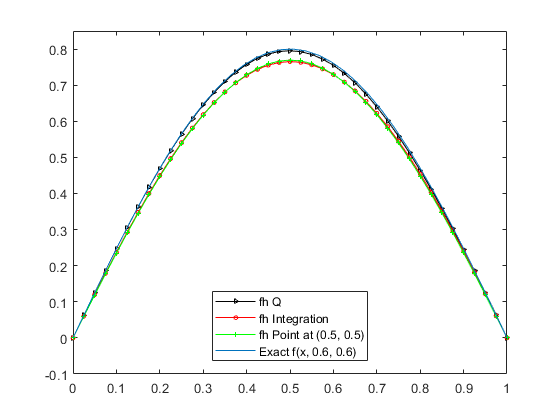
\includegraphics[width=\linewidth]{../FreeFem++/fhx}
	\end{subfigure}%
	\begin{subfigure}{.5\linewidth}
		\centering
		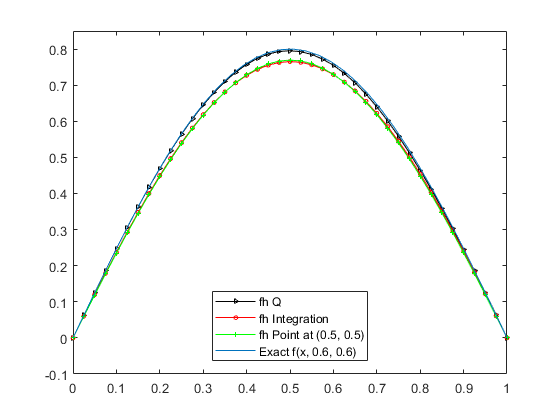
\includegraphics[width=\linewidth]{../FreeFem++/fhx}
	\end{subfigure}
	\caption{The exact and numerical solution of Example 3.1: integral observation (left) and point observation (right).}
\end{figure}
\begin{figure}[h!]
	\begin{subfigure}{.5\linewidth}
		\centering
		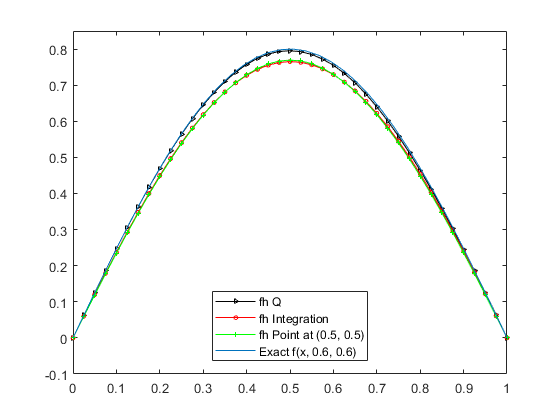
\includegraphics[width=\linewidth]{../FreeFem++/fhx}
	\end{subfigure}%
	\begin{subfigure}{.5\linewidth}
		\centering
		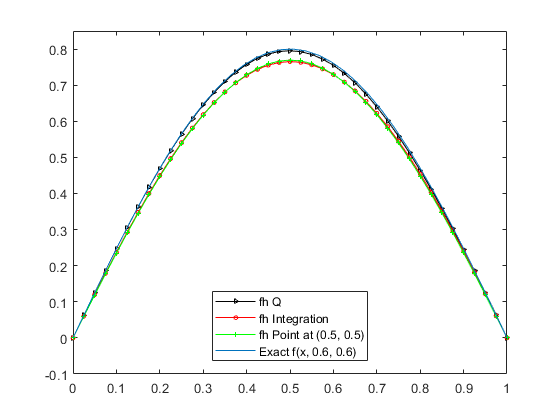
\includegraphics[width=\linewidth]{../FreeFem++/fhx}
	\end{subfigure}
	\caption{The exact and numerical solution of Example 3.2: integral observation (left) and point observation (right).}
\end{figure}

\newpage
\noindent\textbf{Example 2.2}
\\
We reconstruct $f(x)$ with 9 points described as follows
\begin{figure}[h!]
	\begin{subfigure}{.5\linewidth}
		\centering
		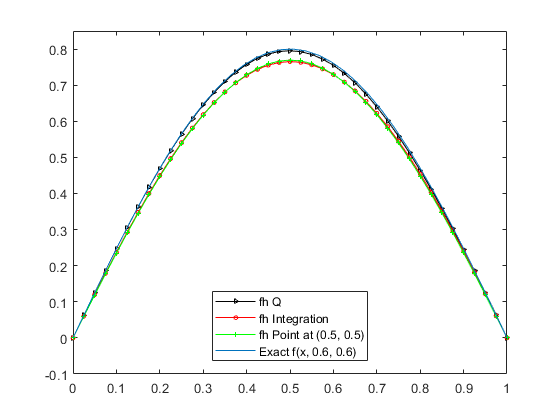
\includegraphics[width=\linewidth]{../FreeFem++/fhx}
	\end{subfigure}%
	\begin{subfigure}{.5\linewidth}
		\centering
		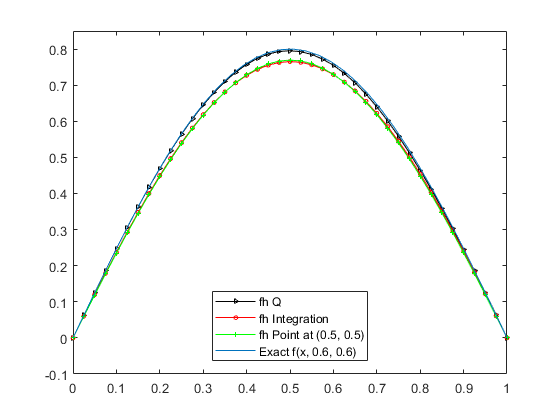
\includegraphics[width=\linewidth]{../FreeFem++/fhx}
	\end{subfigure}
	\caption{Observation points (left) and the exact $f(x_p, t),\;x_p=(0.5, 0.5)$ and numerical solution of Example 2.2 (right).}
\end{figure}\justifying
\section{Conclusion}

\newpage
\bibliography{references}{}
\bibliographystyle{plain}

\end{document}
